\chapter{Introduzione}\label{cap:introduzione}

\section{Contesto}\label{sez:contesto}

A seguito della crescita esponenziale del web in questo secolo e dell'abituarsi di tutti coloro che ne usufruiscono ad un livello grafico sempre migliore e ad una esperienza mano a mano pi\`u interattiva e vicina all'utente medio, i siti web e le tecnologie utilizzate si sono adattati per permettere uno sviluppo sempre pi\`u rapido di codice pi\`u facilmente testabile e mantenibile.

Di conseguenza nel frontend si sono susseguiti una serie di framework e di strumenti, a partire da JQuery\cite{jquery} nel 2006, che per primo si \`e occupato di risolvere il problema della compatibilit\`a tra browsers, permettendo ai developers di scrivere una volta, e poter eseguire su tutti i browsers.

AngularJS nel 2010 \`e stato il primo MVC framework ad offrire in un unico pacchetto un insieme di features che hanno facilitato tantissimo la vita ai developers, come il two-way data binding, la dependency injection, il routin, oltre ad altri strumenti utili per rendere pi\`u standard lo sviluppo nel frontend~\cite{Hoff}.
Questo framework largamente utilizzato, \'e stato riscritto nel 2013 diventando Angular 2 (e nelle versioni pi\'u recenti rinominato semplicemente in Angular) senza mantenere retrocompatibilit\`a e senza offrire un modo preciso per migrare alla nuova versione agli utilizzatori di AngularJS.
Anche per questo React, un nuovo framework pi\`u leggero e modulare sviluppato dagli sviluppatori di Facebook, ha preso il posto di Angular come framework pi\`u utilizzato nel frontend.

Vue infine \'e il terzo dei principali framework che ha provato a prendere piede proponendo una versione intermedia tra il fortemente opinionato Angular e il pi\'u flessibile React.

Oltre a questi, ciascuno con la propria semantica, organizzazione logica dei folder, spesso una CLI dedicata, ad un developer frontend viene solitamente richiesto di conoscere HTML, CSS e chiaramente Javascript essendo ci\'o su cui si basano poi i vari framework.

Oltre a Javascript, se si vuole scrivere degli unit test facilmente mantenibili, bisogna conoscere TypeScript(specialmente se si utilizza Angular, che rende il suo utilizzo obbligatorio) e degli altri framework che facilitino i test(Enzyme, Karma + Jasmine, ...).

\section{Problema}\label{sez:problema}
I continui cambiamenti nei molti framework utilizzati, la diversit\`a degli strumenti stessi tra loro, che spesso realizzano in modo diverso tutti la stessa cosa, rendono sempre pi\'u difficile per un junior developer iniziare a sviluppare, vista l'ampia curva di apprendimento e lo studio necessario, per poter essere spendibile a livello professionale.

Oltretutto un web developer ad oggi finisce per essere costretto a scegliere se diventare uno sviluppatore frontend o backend, dato che rimanere al passo e aggiornarsi gi\`a in solo uno di questi due campi richiede tempo e non \`e scontato ad esempio che venga concesso di poterlo fare in orario lavorativo, pur essendo fondamentale.

\'E quindi chiaro che per tutti i web developer, e specialmente per una figura mista spesso identificata con il titolo "Full-Stack Developer", ci sia una continua ricerca del modo per rendere le proprie competenze quanto pi\'u trasversali possibile, anche in termini di tecnologia utilizzata.

\pagebreak

\section{Linguaggi General-Purpose}\label{sez:problema}
Microsoft, nel backend e in ambito applicativo, ha reso nel tempo il framework .NET e le sue implementazioni(.NET Core, .NET Framework e Mono) utilizzabili nei vari propri linguaggi, C\#, F\# e VB.
La figura 1.1 qui di seguito riassume le implementazioni del .NET Standard e le varie tipologie di applicazioni che si possono sviluppare con ciascuna.

\begin{figure}[H]
	\centerline{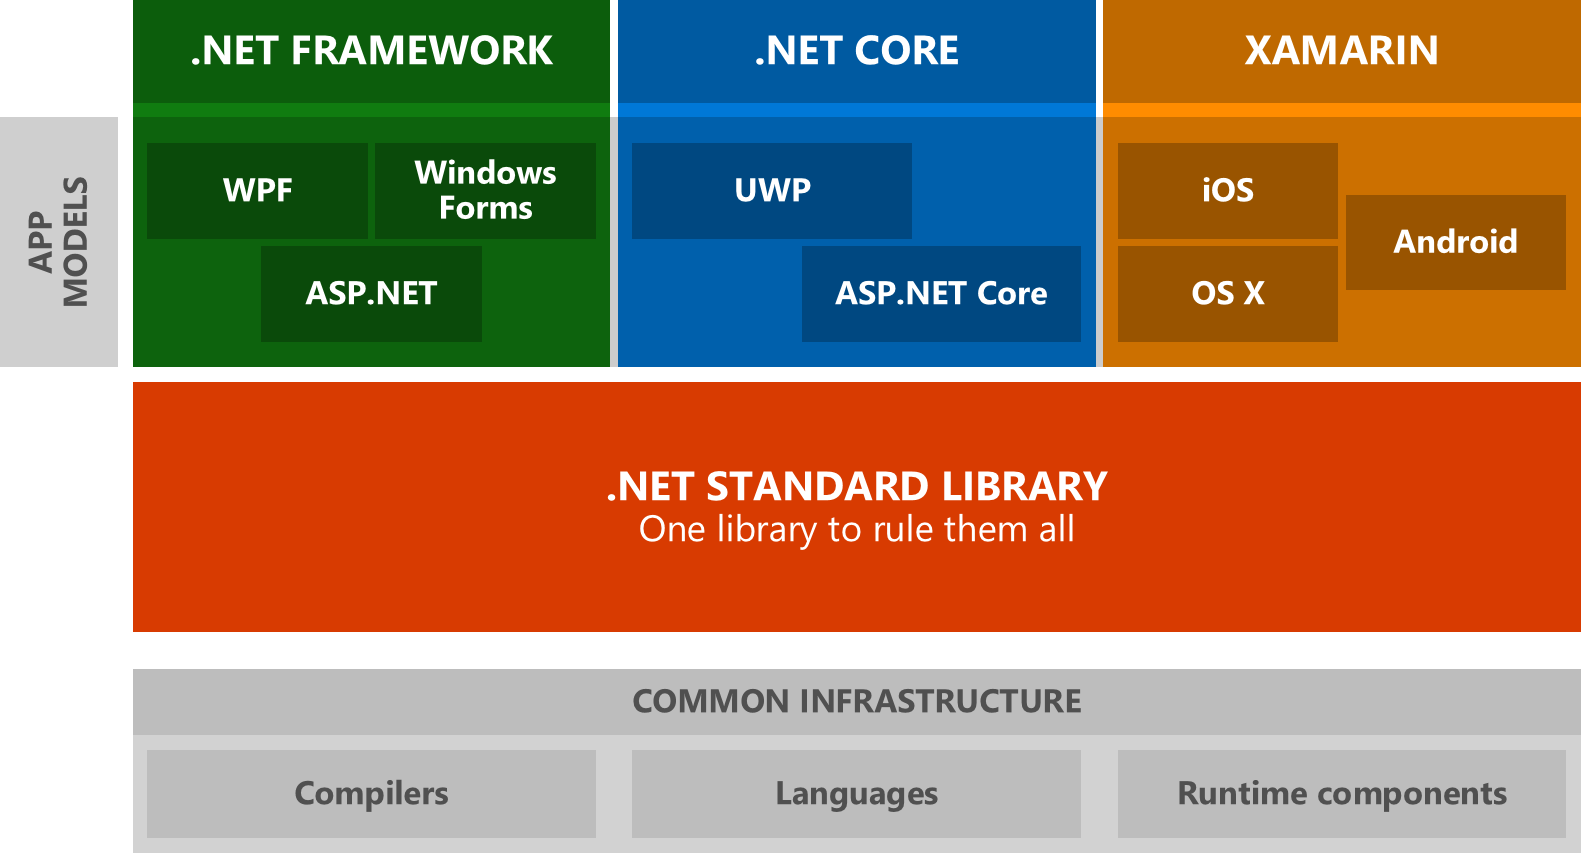
\includegraphics[scale=0.2]{figure/DotNetImplementations}}
	\caption{Implementazioni del .NET Standard}
	\label{fig:DotNetImplementations}
\end{figure}

Scrivendo ad esempio in C\# \`e possibile sviluppare vari tipi di applicazioni come si pu\'o vedere nella figura 1.2, ma se si decide di sviluppare codice per un applicazione client web ad oggi si \`e ancora costretti a scrivere utilizzando Javascript e un suo framework se si vuole essere veloci nello sviluppo e scrivere codice mantenibile specialmente in team pi\'u grandi, come nel mondo enterprise.

\begin{figure}[H]
\centerline{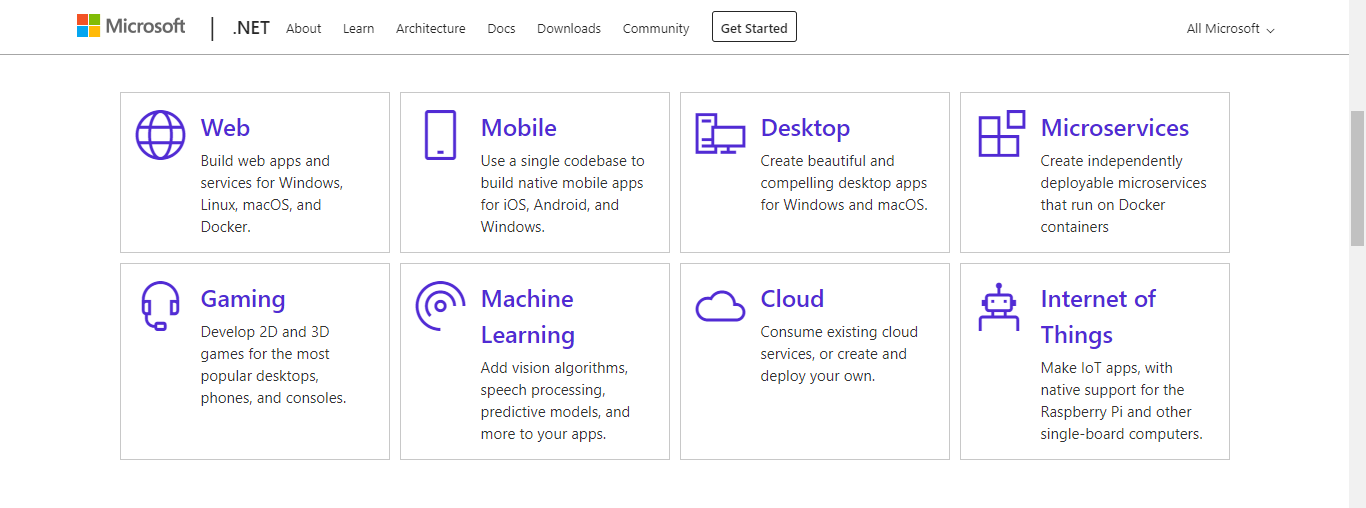
\includegraphics[scale=0.35]{figure/DotNetFrameworkCapabilities}}
\caption{Possibilit\'a di .NET}
\label{fig:DotNetCapabilities}
\end{figure}

Gi\'a con Razor\cite{razor}, Microsoft ha permesso la generazione di codice HTML e CSS in modo dinamico utilizzando C\#, ma \`e utilizzabile solo lato server e quindi la cattura di un evento client side come il click di un utente su un bottone, senza contattare il server, non \`e stato possibile fino ad ora senza passare per Javascript.

\section{Blazor}
Ecco cosa \'e quindi Blazor: la versione pi\'u avanzata di Razor(Browser+Razor\cite{blazorWikiGitHub}) che permette ai developer di gestire anche gli eventi client-side, direttamente in C\#(o nel linguaggio scelto tra quelli supportati) come se questo fosse effettivamente ci\'o che viene eseguito lato client, mentre in reat\'a l'esecuzione lato client cambia a seconda del modello scelto, come poi vedremo pi\'u nel dettaglio.

Blazor utilizza per i vari modelli, delle tecnologie diverse(ad esempio il WebAssembly) ma che rispettano sempre lo standard del web.
Non \'e invece un plugin da installare, e non dipende da un browser specifico.
Non \'e nemmeno una "semplice" tecnologia di transpilazione verso javascript, contrariamente a tecnologie come TypeScript.